% -*- Mode:TeX -*-

%% IMPORTANT: The official thesis specifications are available at:
%%            http://libraries.mit.edu/archives/thesis-specs/
%%
%%            Please verify your thesis' formatting and copyright
%%            assignment before submission.  If you notice any
%%            discrepancies between these templates and the 
%%  z          MIT Libraries' specs, please let us know
%%            by e-mailing thesis@mit.edu

%% The documentclass options along with the pagestyle can be used to generate
%% a technical report, a draft copy, or a regular thesis.  You may need to
%% re-specify the pagestyle after you \include  cover.tex.  For more
%% information, see the first few lines of mitthesis.cls. 

%\documentclass[12pt,vi,twoside]{mitthesis}
%%
%%  If you want your thesis copyright to you instead of MIT, use the
%%  ``vi'' option, as above.
%%
%\documentclass[12pt,twoside,leftblank]{mitthesis}
%%
%% If you want blank pages before new chapters to be labelled ``This
%% Page Intentionally Left Blank'', use the ``leftblank'' option, as
%% above. 

\documentclass[12pt,twoside]{mitthesis}
\usepackage{lgrind}
\usepackage{graphicx}
\usepackage{array}
\usepackage{amsmath}
\usepackage{tikz}
\usepackage{wasysym}
\usepackage{textcomp}
\usepackage{upgreek}


\usetikzlibrary{shapes,arrows}
\newcommand{\unit}[1]{\ensuremath{\, \mathrm{#1}}}
\newcommand{\micron}{\textmu m}

% Define block styles
\tikzstyle{decision} = [diamond, draw, fill=blue!20, 
    text width=4.5em, text badly centered, node distance=3cm, inner sep=0pt]
\tikzstyle{block} = [rectangle, draw, fill=blue!20, 
    text width=6em, text centered, rounded corners, minimum height=4em]
\tikzstyle{line} = [draw, -latex']
\tikzstyle{cloud} = [draw, ellipse,fill=red!20, node distance=3cm,
    minimum height=4em, text width=6em, text centered]

\usepackage{breqn}

\usepackage{float}
%\floatstyle{boxed}
%\restylefloat{table}



\pagestyle{plain}

%% This bit allows you to either specify only the files which you wish to
%% process, or `all' to process all files which you \include.

% \typein [\files]{Enter file names to process, (chap1,chap2 ...), or `all' to
% process all files:}
% \def\all{all}
% \ifx\files\all \typeout{Including all files.} \else \typeout{Including only \files.} \includeonly{\files} \fi

\begin{document}

% -*-latex-*-
% 
% For questions, comments, concerns or complaints:
% thesis@mit.edu
% 
%
% $Log: cover.tex,v $
% Revision 1.8  2008/05/13 15:02:15  jdreed
% Degree month is June, not May.  Added note about prevdegrees.
% Arthur Smith's title updated
%
% Revision 1.7  2001/02/08 18:53:16  boojum
% changed some \newpages to \cleardoublepages
%
% Revision 1.6  1999/10/21 14:49:31  boojum
% changed comment referring to documentstyle
%
% Revision 1.5  1999/10/21 14:39:04  boojum
% *** empty log message ***
%
% Revision 1.4  1997/04/18  17:54:10  othomas
% added page numbers on abstract and cover, and made 1 abstract
% page the default rather than 2.  (anne hunter tells me this
% is the new institute standard.)
%
% Revision 1.4  1997/04/18  17:54:10  othomas
% added page numbers on abstract and cover, and made 1 abstract
% page the default rather than 2.  (anne hunter tells me this
% is the new institute standard.)
%
% Revision 1.3  93/05/17  17:06:29  starflt
% Added acknowledgements section (suggested by tompalka)
% 
% Revision 1.2  92/04/22  13:13:13  epeisach
% Fixes for 1991 course 6 requirements
% Phrase "and to grant others the right to do so" has been added to 
% permission clause
% Second copy of abstract is not counted as separate pages so numbering works
% out
% 
% Revision 1.1  92/04/22  13:08:20  epeisach

% NOTE:
% These templates make an effort to conform to the MIT Thesis specifications,
% however the specifications can change.  We recommend that you verify the
% layout of your title page with your thesis advisor and/or the MIT 
% Libraries before printing your final copy.

%\title{A Fiber Based Optical Coherence Tomography System for Analyzing Cochlear Motion}

\title{Design and Implementation of a Fiber Optic Doppler Optical Coherence Microscopy System for Cochlear Imaging}

\author{Logan Patrick Williams}
% If you wish to list your previous degrees on the cover page, use the 
% previous degrees command:
%       \prevdegrees{A.A., Harvard University (1985)}
% You can use the \\ command to list multiple previous degrees
%       \prevdegrees{B.S., University of California (1978) \\
%                    S.M., Massachusetts Institute of Technology (1981)}
\department{Department of Electrical Engineering and Computer Science}

% If the thesis is for two degrees simultaneously, list them both
% separated by \and like this:
% \degree{Doctor of Philosophy \and Master of Science}
\degree{Master of Engineering in Electrical Science and Engineering}

% As of the 2007-08 academic year, valid degree months are September, 
% February, or June.  The default is June.
\degreemonth{June}
\degreeyear{2014}
\thesisdate{May 23, 2014}

%% By default, the thesis will be copyrighted to MIT.  If you need to copyright
%% the thesis to yourself, just specify the `vi' documentclass option.  If for
%% some reason you want to exactly specify the copyright notice text, you can
%% use the \copyrightnoticetext command.  
%\copyrightnoticetext{\copyright IBM, 1990.  Do not open till Xmas.}

% If there is more than one supervisor, use the \supervisor command
% once for each.
\supervisor{Dennis M. Freeman}{Dean for Undergraduate Education}

% This is the department committee chairman, not the thesis committee
% chairman.  You should replace this with your Department's Committee
% Chairman.
\chairman{Arthur C. Smith}{Chairman, Department Committee on Graduate Theses}

% Make the titlepage based on the above information.  If you need
% something special and can't use the standard form, you can specify
% the exact text of the titlepage yourself.  Put it in a titlepage
% environment and leave blank lines where you want vertical space.
% The spaces will be adjusted to fill the entire page.  The dotted
% lines for the signatures are made with the \signature command.
\maketitle

% The abstractpage environment sets up everything on the page except
% the text itself.  The title and other header material are put at the
% top of the page, and the supervisors are listed at the bottom.  A
% new page is begun both before and after.  Of course, an abstract may
% be more than one page itself.  If you need more control over the
% format of the page, you can use the abstract environment, which puts
% the word "Abstract" at the beginning and single spaces its text.

%% You can either \input (*not* \include) your abstract file, or you can put
%% the text of the abstract directly between the \begin{abstractpage} and
%% \end{abstractpage} commands.

% First copy: start a new page, and save the page number.
\cleardoublepage
% Uncomment the next line if you do NOT want a page number on your
% abstract and acknowledgments pages.
% \pagestyle{empty}
\setcounter{savepage}{\thepage}
\begin{abstractpage}
% $Log: abstract.tex,v $
% Revision 1.1  93/05/14  14:56:25  starflt
% Initial revision
% 
% Revision 1.1  90/05/04  10:41:01  lwvanels
% Initial revision
% 
%
%% The text of your abstract and nothing else (other than comments) goes here.
%% It will be single-spaced and the rest of the text that is supposed to go on
%% the abstract page will be generated by the abstractpage environment.  This
%% file should be \input (not \include 'd) from cover.tex.

In this thesis, the design and implementation of a fiber optic Doppler optical coherence microscopy (FO-DOCM) system for cochlear imaging applications is presented. The use of a fiber optic design significantly reduces system size and complexity and the construction of a novel alignment and micropositioning apparatus increases ease of use for the researcher performing the imaging. To enable precise motion measurements, a time domain DOCM approach is used, utilizing an acousto-optic modulator (AOM) based optical heterodyne system to generate a stationary interference carrier frequency. By referencing this interference signal against the AOM drive signals, precise measurements of motions with magnitude on the order of $10$ pm are shown to be possible. In addition to interferometrically measuring small amplitude motion, the FO-DOCM system is shown to be capable of imaging with a volumetric resolution of $10 \times 9 \times 9$ \micron. Demonstrative results of imaging cochlear tissue are presented by using the FO-DOCM to image and measure motion in a guinea pig cochlea {\em in vitro}.

% In this thesis, I designed and implemented a compiler which performs
% optimizations that reduce the number of low-level floating point operations
% necessary for a specific task; this involves the optimization of chains of
% floating point operations as well as the implementation of a ``fixed'' point
% data type that allows some floating point operations to simulated with integer
% arithmetic.  The source language of the compiler is a subset of C, and the
% destination language is assembly language for a micro-floating point CPU.  An
% instruction-level simulator of the CPU was written to allow testing of the
% code.  A series of test pieces of codes was compiled, both with and without
% optimization, to determine how effective these optimizations were.

\end{abstractpage}

% Additional copy: start a new page, and reset the page number.  This way,
% the second copy of the abstract is not counted as separate pages.
% Uncomment the next 6 lines if you need two copies of the abstract
% page.
% \setcounter{page}{\thesavepage}
% \begin{abstractpage}
% % $Log: abstract.tex,v $
% Revision 1.1  93/05/14  14:56:25  starflt
% Initial revision
% 
% Revision 1.1  90/05/04  10:41:01  lwvanels
% Initial revision
% 
%
%% The text of your abstract and nothing else (other than comments) goes here.
%% It will be single-spaced and the rest of the text that is supposed to go on
%% the abstract page will be generated by the abstractpage environment.  This
%% file should be \input (not \include 'd) from cover.tex.

In this thesis, the design and implementation of a fiber optic Doppler optical coherence microscopy (FO-DOCM) system for cochlear imaging applications is presented. The use of a fiber optic design significantly reduces system size and complexity and the construction of a novel alignment and micropositioning apparatus increases ease of use for the researcher performing the imaging. To enable precise motion measurements, a time domain DOCM approach is used, utilizing an acousto-optic modulator (AOM) based optical heterodyne system to generate a stationary interference carrier frequency. By referencing this interference signal against the AOM drive signals, precise measurements of motions with magnitude on the order of $10$ pm are shown to be possible. In addition to interferometrically measuring small amplitude motion, the FO-DOCM system is shown to be capable of imaging with a volumetric resolution of $10 \times 9 \times 9$ \micron. Demonstrative results of imaging cochlear tissue are presented by using the FO-DOCM to image and measure motion in a guinea pig cochlea {\em in vitro}.

% In this thesis, I designed and implemented a compiler which performs
% optimizations that reduce the number of low-level floating point operations
% necessary for a specific task; this involves the optimization of chains of
% floating point operations as well as the implementation of a ``fixed'' point
% data type that allows some floating point operations to simulated with integer
% arithmetic.  The source language of the compiler is a subset of C, and the
% destination language is assembly language for a micro-floating point CPU.  An
% instruction-level simulator of the CPU was written to allow testing of the
% code.  A series of test pieces of codes was compiled, both with and without
% optimization, to determine how effective these optimizations were.

% \end{abstractpage}

\cleardoublepage

\section*{Acknowledgments}

%% Dedicated to the memory of my father, who taught me how to listen.

Thanks to Professor Denny Freeman, for taking me an as a student, privileging me with the power and responsibility to make my own mistakes, and encouraging my progress whenever I felt overwhelmed.

Thanks to Scott Page, Jon Sellon, and Shirin Farrahi for their support, advice, and unending help with everything, from finding what I needed around the lab, to debugging optical systems, to preparing the samples used to test the FO-DOCM apparatus.

Thanks to Rooz Ghaffari, for introducing me to the Micromechanics Group.

Thanks to Janice Balzer for her help and organization around the Micromechanics Group.

Thanks to my friends in and around MIT for your support and camaraderie. MIT would not have been possible without you.

Thanks to my mother Lorie, and my brother Aaron, for your constant love and understanding.

Finally, thanks to my father Steve, to whose memory I dedicate this work. You gave me music -- you gave me everything.

%%%%%%%%%%%%%%%%%%%%%%%%%%%%%%%%%%%%%%%%%%%%%%%%%%%%%%%%%%%%%%%%%%%%%%
% -*-latex-*-

% Some departments (e.g. 5) require an additional signature page.  See
% signature.tex for more information and uncomment the following line if
% applicable.
% % -*- Mode:TeX -*-
%
% Some departments (e.g. Chemistry) require an additional cover page
% with signatures of the thesis committee.  Please check with your
% thesis advisor or other appropriate person to determine if such a 
% page is required for your thesis.  
%
% If you choose not to use the "titlepage" environment, a \newpage
% commands, and several \vspace{\fill} commands may be necessary to
% achieve the required spacing.  The \signature command is defined in
% the "mitthesis" class
%
% The following sample appears courtesy of Ben Kaduk <kaduk@mit.edu> and
% was used in his June 2012 doctoral thesis in Chemistry. 

\begin{titlepage}
\begin{large}
This doctoral thesis has been examined by a Committee of the Department
of Chemistry as follows:

\signature{Professor Jianshu Cao}{Chairman, Thesis Committee \\
   Professor of Chemistry}

\signature{Professor Troy Van Voorhis}{Thesis Supervisor \\
   Associate Professor of Chemistry}

\signature{Professor Robert W. Field}{Member, Thesis Committee \\
   Haslam and Dewey Professor of Chemistry}
\end{large}
\end{titlepage}


\pagestyle{plain}
  % -*- Mode:TeX -*-
%% This file simply contains the commands that actually generate the table of
%% contents and lists of figures and tables.  You can omit any or all of
%% these files by simply taking out the appropriate command.  For more
%% information on these files, see appendix C.3.3 of the LaTeX manual. 
\tableofcontents
\newpage
\listoffigures
\newpage
%\listoftables


%% This is an example first chapter.  You should put chapter/appendix that you
%% write into a separate file, and add a line \include{yourfilename} to
%% main.tex, where `yourfilename.tex' is the name of the chapter/appendix file.
%% You can process specific files by typing their names in at the 
%% \files=
%% prompt when you run the file main.tex through LaTeX.
\chapter{Introduction}

%% Chapter outline goes here

\section{Motivations for a fiber optic DOCM system}

The mammilian cochlea is capable of remarkable sensory perception. It can distinguish motions as small as the radius of a hydrogen atom and discriminate between up to 30 frequencies within a single semitone. \cite{ghafarri} However, the mechanics of motion in the inner ear remain poorly understood. The Micromechanics Group at RLE is  analyzing motion in the cochlea in order to more fully understand what gives rise to these remarkable sensory abilities.

\begin{figure}[h!]
  \centering
    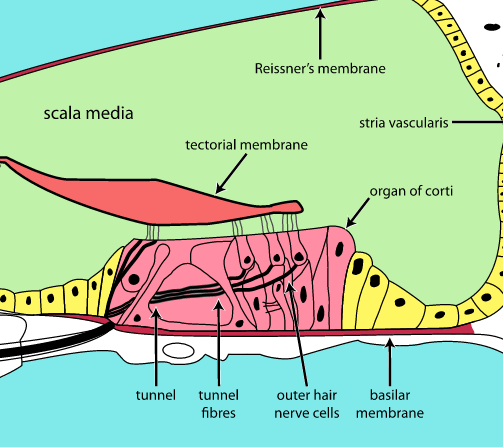
\includegraphics[width=0.8\textwidth]{Images/Background/cochlea.png}
      \caption{A schematic of tissues in the cochlea.}
      \label{fig:cochlea}
\end{figure}

A tissue of particular interest in the cochlea is the tectorial membrane, which is in direct contact with the hair cells, as shown in Figure \ref{fig:cochlea}. This tissue has some interesting mechanical properties, and its position in relation to the sensory cells suggests it could play in active role in motion amplification or in frequency discrimination. However, as it is almost entirely water, it is very difficult to image with conventional imaging techniques.

A technique known as optical coherence tomography allows three-dimensional imaging into tissues, such as the tectorial membrane, by making use of the auto-correlation properties of temporally incoherent light. When used with a high NA lens for high resolution transverse imaging, the technique is also known as optical coherence microscopy. This technique can image deeper into tissues than other three-dimensional imaging methods such as confocal microscopy. Furthermore, OCT allows for measurement of motion (citation here?), both constant and periodic, as will be explained later in the introduction.

The Micromechanics Group at RLE currently uses a doppler optical coherence microscopy, or DOCM (a subset of doppler optical coherence tomography, or DOCT) system to image the mammilian cochlea and acquire data about the mechanical motions of tissues. This system was developed by former student Stanley Hong. \cite{hong}

The current system is designed around free space optics that have been carefully aligned and positioned on an optics table. This design has several disadvantages, chiefly that it is difficult and time consuming to align with the animal that is being imaged. This process can take several hours, due to the need to move the animal precisely under the DOCT objective, and the need to align the cochlea with the fixed optical axis of the DOCT system. Furthermore, the current free space system is bulky and fragile.

The system described in this thesis, while similar in many ways to the existing DOCT system, primarily uses fiber optic coupled components. Fiber optics can be more compact, and are almost insensitive to movement or changes in physical shape (one notable exception to this, with regards to polarization, will be discussed in Chapter 2). Additionally, the objective used for imaging the actual tissue is mounted on a custom designed mechanical apparatus that allows for a variable angle optical axis, and easy repositioning, to work with the researcher and research animal, rather than forcing the animal to conform to the optical system. These improvements should significantly improve the workflow of other researchers in the Micromechanics Group.

\section{Principle of operation of time domain OCT}
\label{sec:principles_oct}

Throughout this document, the coordinate axis parallel to the direction of light emission from the objective shall be referred to as the ``axial'' direction, or ``z'' axis. The plane perpendicular to this axis is known as the ``transverse'' plane, or, sometimes, the ``x'' and ``y'' axes.

\begin{figure}[h!]
\centering
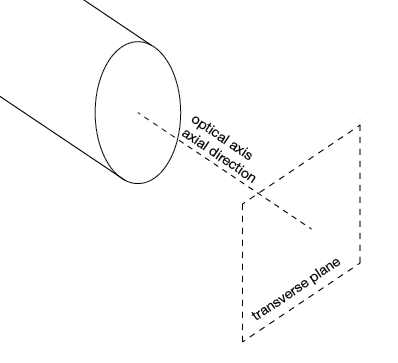
\includegraphics[width=0.6\textwidth]{Images/Background/axes.png}
\caption{Definition of axes.}
\end{figure}

\begin{figure}[h!]
  \centering
    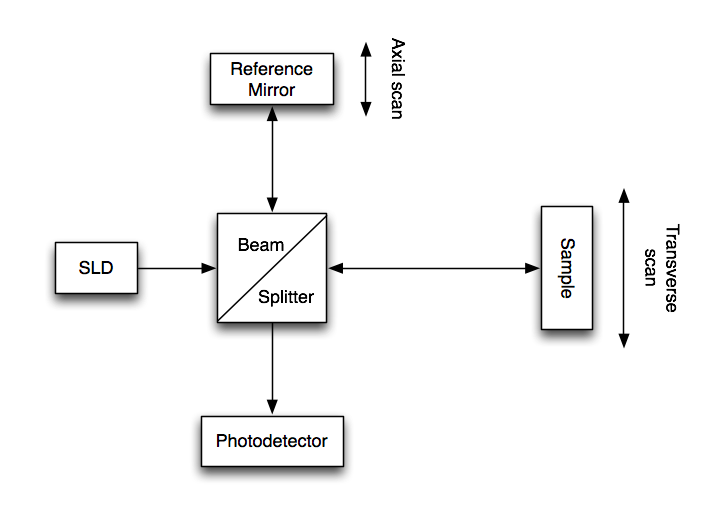
\includegraphics[width=0.8\textwidth]{Images/Background/basic_oct.png}
      \caption{A schematic of a basic OCT system.}
\end{figure}


OCT functions by utilizing the principle of the Michelson interferometer, as shown in Figure 1. Light is split in to two beams. One is reflected from a mirror, the other is scattered from a biological sample. The light is then recombined and the intensity measured by a photodetector. When the optical path lengths of the two beams are closely matched, and interference pattern may be observed. By using temporally incoherent (broadband) light, the interference pattern is capable of absolute localization.

The electric field from a temporally incoherent source can be modeled accurately as a wide-sense stationary random process with a certain power spectral density. \cite{Bouma} In the case where the scattering sample is replaced by a reflecting mirror, the mathematical analysis may be simplified greatly by assuming that two time delayed versions of this processes are being interfered. From this, we show that interference is the same as autocorrelation, and make use of the Wiener-Khinchin theorem. This derivation follows closely that of Fercher et. al. \cite{fercher}

The intensity of light with analytic (complex) amplitude $V(t)$ is defined as:

\begin{equation}
I(t) = V^*(t)V(t)
\end{equation}

In an OCT system, the light from a reference path is combined with the light from a sample path after some delay. We may express this as:

\begin{equation}
V_D(t; \Delta t) = V_S(t) + V_R(t + \Delta t)
\end{equation}

Of course, since measuring instantaneous electric field amplitude is impossible, we are interested in ensemble averages of intensity. This gives the following result, where $\Gamma_{XY}$ represents the cross correlation between two random processes $X$ and $Y$.

\begin{equation}
\begin{aligned}
\bar{I}_E(\Delta t) & =  \langle I_E(t; \Delta t) \rangle \\
& =  \langle V^*_E(t; \Delta t) V_E(t; \Delta t) \rangle \\
& =  \langle I_S(t) \rangle + \langle I_R(t) \rangle + 2 \Re \{\Gamma_{SR} (\Delta t) \}
\end{aligned}
\end{equation}

$\Delta t$ is proportional to the path length difference between the two beams, $\Delta t = \Delta z / c$. When both sample and reference paths are illuminated from the same light source, the cross correlation function above simplifies into an autocorrelation function of the light source. From here, the Wiener-Khinchin theorem can be applied, which states that the autocorrelation function of a wide-sense stationary random process is related to the process power spectral density by a Fourier transform.

\begin{equation}
\Gamma_{XX}(\tau) = 2 \int_{0}^\infty S_{XX}(f) \exp(2 \pi j \tau f) \,df
\end{equation}

Therefore, the axial resolution in an OCT system is limited by the spectral properties of the light source. Given a source of center wavelength $\lambda_0$ and bandwidth $\Delta \lambda$, if we assume a Gaussian PSD, we may find the width of the autocorrelation function, and therefore the axial resolution. \cite{fercher}

\begin{equation} \label{eq:ares}
\delta_z = l_c = \frac{2 \ln{2}}{\pi} \frac{\lambda_0^2}{\Delta \lambda}
\end{equation}

This however, is just the envelope of the autocorrelation function. It is also modulated by a carrier, with a  frequency dependent on the wavelength of the light source, $\lambda_0$, and the speed of the scan, $v_s$. \cite{fercher}

\begin{equation} \label{eq:carrier}
f_{mod} = 4 \pi v_s / \lambda_0
\end{equation}

The transverse resolution is the standard diffraction limit for a lens. \cite{hecht}

\begin{equation} \label{eq:tres}
\delta_x = 0.61 \frac{\lambda}{NA}
\end{equation}

\section{Heterodyne OCT with Acousto-optic Modulators}

As derived in the previous section, the frequency of the carrier is dependent on the speed of the z-axis motion. For typical cases, this is on the order of 1 KHz. If the speed of the scan is variable, this carrier is inconsistent, and if the scan stops at a particular point, the frequency is near zero (non-zero only due to mechanical vibration).

In some cases, it is desirable to have a higher carrier frequency, or a carrier frequency that is independent of the speed of the z-axis scan. This can also be useful for cases where the z speed is zero, as in \begin{em}en-face\end{em} OCT. \cite{bouma}

\subsection{Principle of operation of acousto optic modulators}

\begin{figure}[h!]
\centering
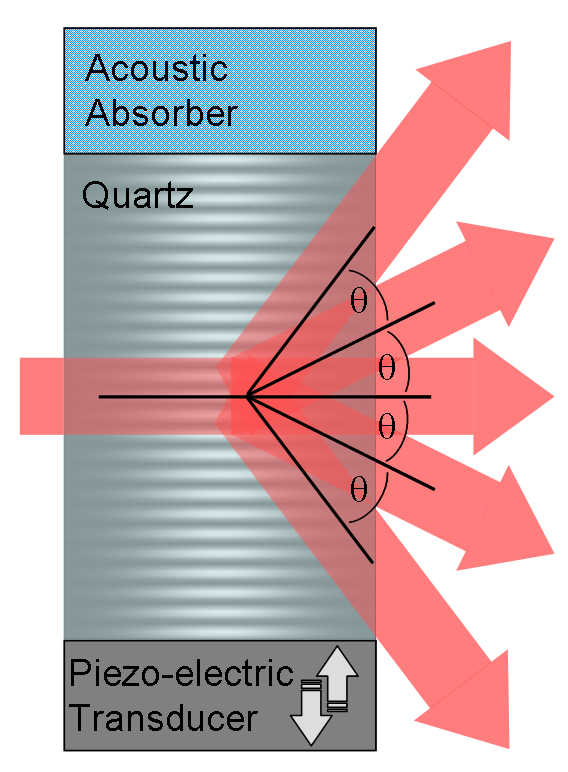
\includegraphics[width=0.3\textwidth]{Images/Background/aom.png}
\caption{Light scatters off of acoustic waves in a quartz crystal, changing both frequency and angle.}
\end{figure}

Acousto optic modulators (AOMs) are crystals, typically quartz, that use acousto-optic effect to shift the frequency of light. A transducer establishes an acoustic standing wave at RF frequencies inside the crystal. Compression waves in the crystal can be modeled as gradients in the refractive index. [McCarron] Light incident upon these refractive index gradients will be scattered.

\begin{figure}[h!]
\centering
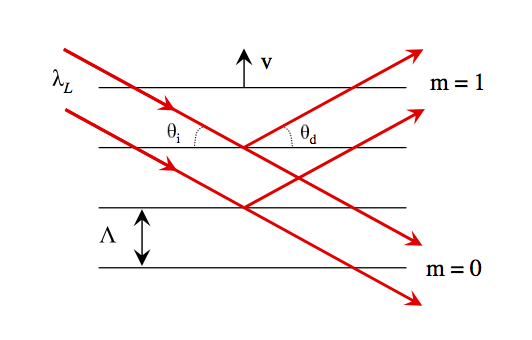
\includegraphics[width=0.5\textwidth]{Images/Background/aom_scattering.png}
\caption{Light scattering off of acoustic wavefronts in an acousto-optic modulator.}
\end{figure}

Scattered light interferes constructively when the following condition is met.

\begin{equation} \label{eq:constructive_interference}
n \lambda_L = \Lambda (\sin{\theta_i} + \sin{\theta_d})
\end{equation}

Conservation of momentum requires that $\theta_i = \theta_d$, which simplifies the constructive interference condition to:

\begin{equation}
n \lambda_L = 2 \Lambda \sin{\theta_d}
\end{equation}


This Bragg diffraction also shifts the frequency of the light up by $mF$, where $m$ is the order of diffraction, and $F$ is the acoustic wave frequency.

In a fiber-coupled AOM, the input and output fibers are aligned with the first order diffraction beam.

\subsection{Generating a carrier wave with AOMs}
\label{sec:aom_carrier}

Even with an imprecise or drifting optical frequency, the precise shift frequency induced by an AOM can be used to generate an extremely stable optical interference signal.

The instantaneous complex electric field can be written for two different frequencies can be written as

\begin{align}
E_a(t) & = E_a e^{2 \pi ft j} \\
E_b(t) & = E_b e^{2 \pi (f + F)t j}
\end{align}

The interference between these two fields creates a beat frequency, with the optical frequency amplitude modulated by the slower RF frequency $F$.

\begin{align}
E_a(t) + E_b(t) = & E_a e^{2 \pi ftj} + E_b e^{2 \pi (f + F)t j} \\
= & E_a e^{2 \pi ft j} + E_b (e^{2 \pi ftj} e^{2 \pi Ftj}) \\
= & e^{2 \pi ftj} (E_a + E_b e^{2 \pi Ftj}) \\
= & E_a(t) (1 + \frac{E_a}{E_b} e^{2 \pi Ftj})
\end{align}

The RF frequency $F$ used to drive the AOMs is typically on the order of 40-200 MHz. For many applications, this is a higher carrier frequency than desired. In this case, it is possible to use two AOMs to generate an even lower frequency carrier, by driving them at slightly different RF frequencies.

\begin{align}
E_a(t) & = E_a \exp{(2 \pi t j (f + F_1))} \\
E_b(t) & = E_b \exp{(2 \pi t j (f + F_2))}
\end{align}

It can be seen via an identical simplification to the above that the combination of these electric field amplitudes creates a carrier wave with frequency equal to the absolute value of $F_1 - F_2$.

\section{Doppler OCT with AOMs}

Scattering off of moving particles induces a change in the frequency of scattered light.

%% more equations/background

Excitations and movements of interest are typically sinusoidal in the applications of this OCT device. The instaneous velocity of the scattering media can therefore be written as follows, where $A_o$ is the amplitude of motion and $\omega$ is the acoustic frequency of excitation.

\begin{equation} \label{eq:media_v}
v(t) = A_o \cos{(\omega t)}
\end{equation}

This produces a frequency shift.

%% more equations / background

The new instantaneous electric field amplitudes may be written as follows, and their sum may be calculated.

\begin{align}
E_a(t) & = E_a \exp{(2 \pi t j (f + F_1)(1 + \frac{A_o\cos{\omega t}}{c}))} \\
E_b(t) & = E_b \exp{(2 \pi t j (f + F_2))}
\end{align}

\begin{dmath}
E_b(t) + E_a(t) = E_a \exp{(2 \pi t j (f + F_1))}\left(\exp{\left(\frac{2 \pi t j A_o \cos{wt}}{c}(f + F_1)\right)} + \frac{E_b}{E_a} \exp{(2 \pi t j (F_2 - F_1))}\right)
\end{dmath}

This equation can be simplified slightly by substituting two new symbols for the modified optical frequency and RF frequency difference.

\begin{align*}
f' = & f + F_1 \\
\Delta F = & F_2 - F_1
\end{align*}

\begin{dmath}
E_b(t) + E_a(t) = E_a \exp{(2 \pi t j f')}\left(\exp{\left(2 \pi t j f' \frac{ A_o \cos{wt}}{c}\right)} + \frac{E_b}{E_a} \exp{(2 \pi t j \Delta F)}\right)
\end{dmath}

The instantaneous light intensity is equivalent to the absolute value of the instaneous electric field amplitude squared.

\begin{dmath}
I(t) = E_a^2 \left(1 + \frac{E_b^2}{E_a^2} + 2 \frac{E_b}{E_a} \cos{\left(2 \pi t \left(\Delta F + f' \left( \frac{A_o \cos{\omega t}}{c} \right) \right)\right)} \right)
\end{dmath}

\begin{dmath}
I(t) = E_a^2 + E_b^2 + 2 E_b E_a \cos{\left(2 \pi t \left(\Delta F + f' \left( \frac{A_o \cos{\omega t}}{c} \right)  \right)\right)}
\end{dmath}

The frequency shift induced by the motion of the media can clearly be seen in the instaneous phase of the intensity oscillation.

\begin{dmath}
\phi(t) = 2 \pi t \left(\Delta F + f' \left( \frac{A_o \cos{\omega t}}{c} \right)   \right)
\end{dmath}

This is equivalent to frequency modulation, with the periodic change in frequency of

\begin{equation}
f' \left( \frac{A_o \cos{\omega t}}{c} \right)
\end{equation}


\section{Signal processing}

%% signal processing figure

\begin{figure}[h!]
  \centering
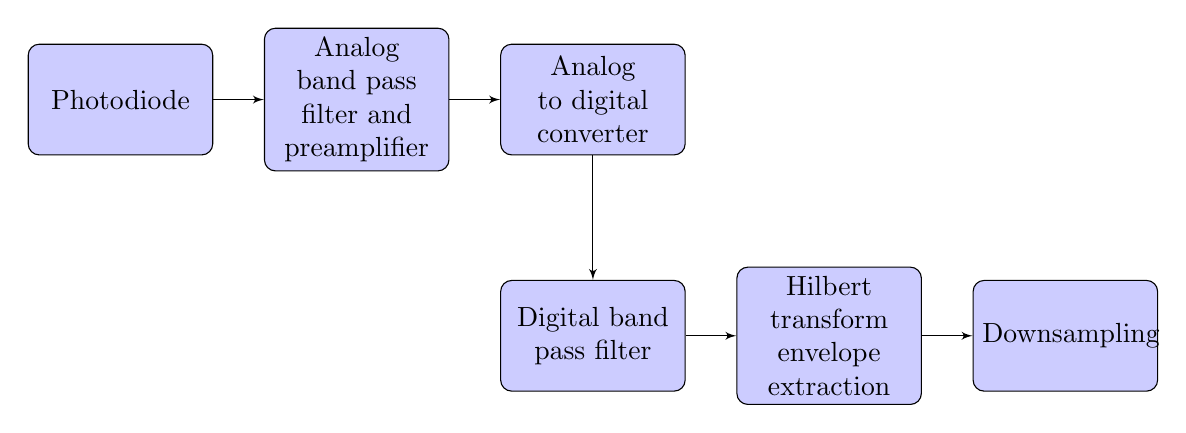
\begin{tikzpicture}[node distance = 2cm, auto]
    % Place nodes
    \node [block] (bpf) {Analog band pass filter and preamplifier};
    \node [block, left of=bpf, node distance=3cm] (pd) {Photodiode};
    \node [block, right of=bpf, node distance=3cm] (adc) {Analog to digital converter};
    \node [block, below of=adc, node distance=3cm] (dbpf) {Digital band pass filter};
    \node [block, right of=dbpf, node distance=3cm] (hilb) {Hilbert transform envelope extraction};
    \node [block, right of=hilb, node distance=3cm] (ds) {Downsampling};
    % Draw edges
    \path [line] (pd) -- (bpf);
    \path [line] (bpf) -- (adc);
    \path [line] (adc) -- (dbpf);
    \path [line] (dbpf) -- (hilb);
    \path [line] (hilb) -- (ds);
\end{tikzpicture}
\caption{Basic OCT signal processing chain. The bandpass filter is centered around the carrier frequency from equation \ref{eq:carrier}. The demodulator either can be as straightforward as an envelope follower or a Hilbert transform based analytic continuation.}
\end{figure}

Prior to analog-to-digital conversion, analog bandpass filters select for the carrier frequency and its sidebands.

The Hilbert transform can be used to extract the envelope from the carrier. Given a signal of the form

\begin{equation}
x(t) = A(t)\cos{(\omega t)}
\end{equation}

the Hilbert transform can generate the quadrature component, given by

\begin{equation}
H(x(t)) \approx A(t) \sin{(\omega t)}
\end{equation}

It can therefore be seen that the envelope component of the signal can be calculated quite easily.

\begin{equation}
A(t) \approx \sqrt{(x(t))^2 + H(x(t))^2}
\end{equation}

The envelope, which does need the high sampling rate previously required in order to capture the carrier frequency, can then be downsampled to the resolution required by the imaging

\section{Literature review}

Hong
Mendeley

\chapter{System design}

In this chapter, the major components of the fiber optic doppler optical coherence microscopy system will be introduced, and the design constraints that led to their choice will be examined. The mechanical and optical design will be detailed. Finally, predictions of system performance will be made based on component choices.

\section{System overview}

\begin{figure}[h!]
\centering
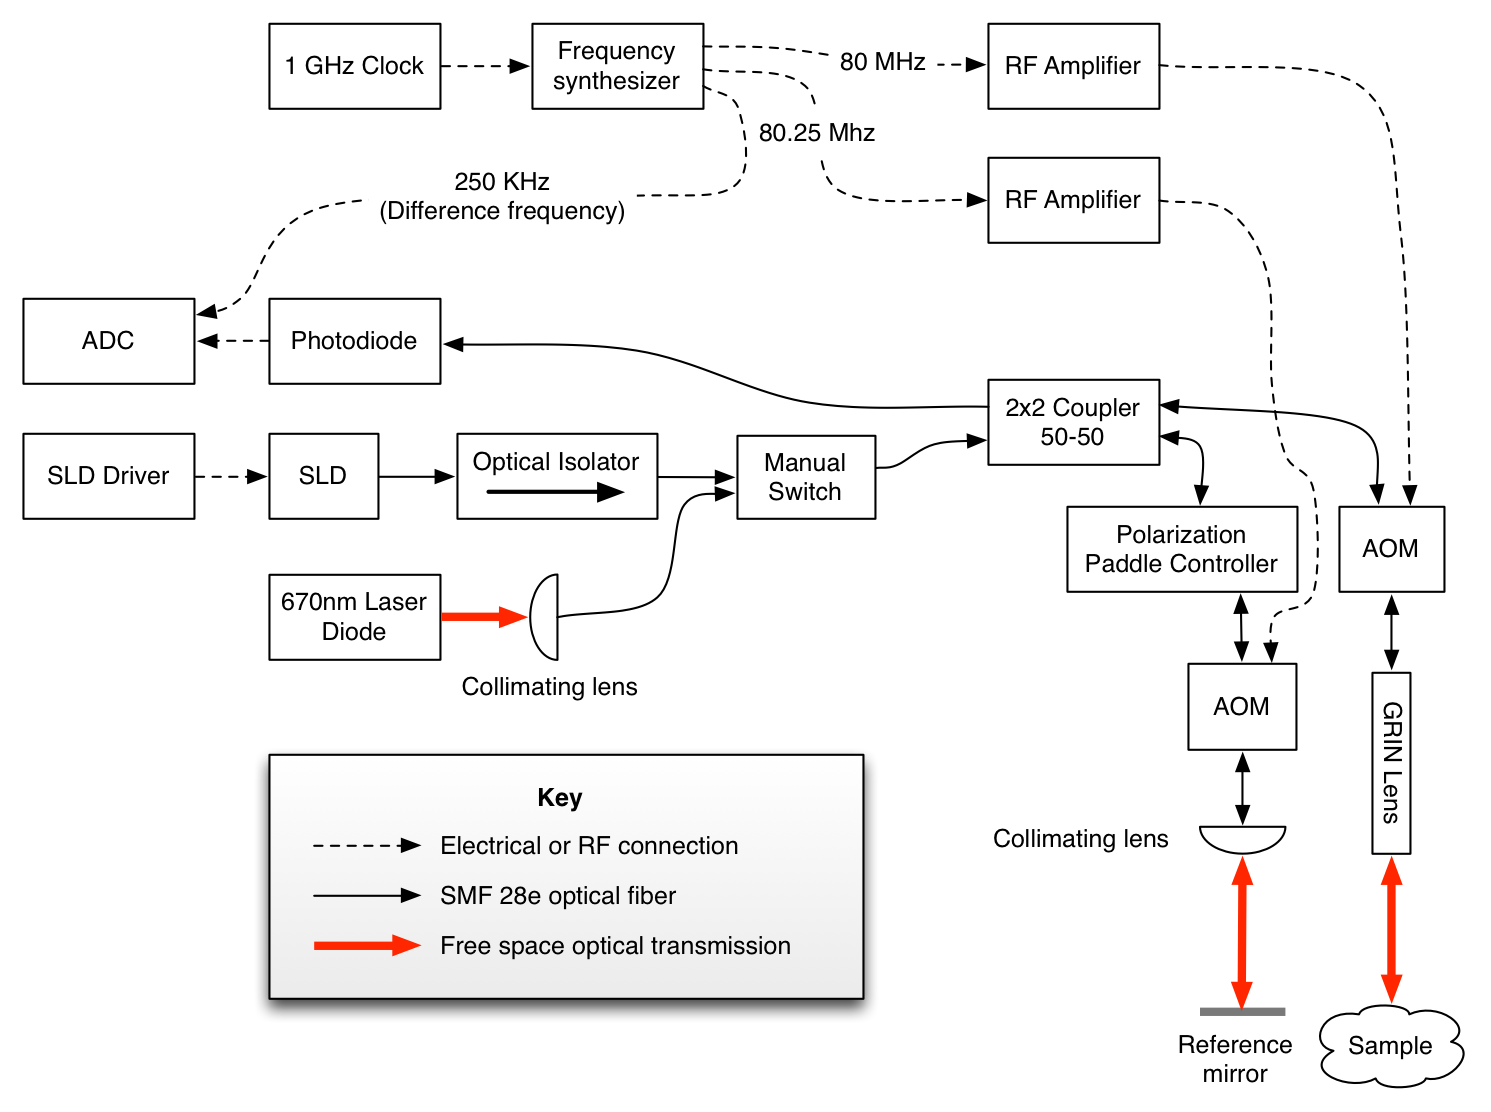
\includegraphics[width=1.1\textwidth]{Images/Background/actual_system_vertical.png}
\caption{Block diagram showing the major components in the fiber optic DOCM system.}
\end{figure}

\subsection{Incoherent light source}

The choice of a light source dictates many aspects of the system performance. The coherence length, as shown in Section~\ref{sec:principles_oct}, controls the axial resolution of the imaging. The center wavelength of the source constrains other components that may be used in the system, the achievable penetration depth, and what tissues may be penetrated, as discussed in Section~\ref{sec:bone}.

For this project,  an Exalos super-luminescent diode (SLD) was choosen. Super luminescent diodes provide the spatial coherence of a laser with the temporal incoherence (therefore, short coherence length) of an LED or ``white'' light source.

A center wavelenght of 1310 nm was choosen as this is a common wavelength for communications. It is therefore possible to find many inexpensive fiber coupled components designed to operate in this band.

\begin{table}[h!]
\centering
\begin{tabular}{ >{\bf}r | l}
Part number & Exalos EXS210045-01 \\
Center wavelength & 1310 nm \\
FWHM Bandwidth & 100 nm \\
Coherence length & 7.57 $\mu$m \\
Power & 10 mW \\
Price & \$1800, \$900 driver \\
\end{tabular}
\caption{Specifications for the optical source.}
\end{table} 

\subsection{Acousto-optic modulators}

Two Gooch \& Housego acousto-optic modulators were choosen. Sintec Optronics packages these AOMs in a fiber coupled enclosed package, which avoided the need for alignment with the first degree deflection beam, and provides a convenient, compact device. An 80 MHz drive frequency was choosen for compatibility with existing hardware used in the Micromechanics group. Detailed specifications for this device are shown in Table 2.2.

\begin{table}[h!]
\centering
\begin{tabular}{ >{\bf}r | l}
Part number & \\
Center wavelength & 1310 nm \\
-3dB Bandwidth & 100 nm \\
Drive frequency & 80 MHz \\
Drive power & 1.5 W \\
Price & 2, at \$1500 each \\
\end{tabular}
\caption{Specifications for the acousto-optic modulator.}
\end{table} 

\subsection{RF Generation and Driving}

The AOMs need to be driven by an 80 Mhz and an 80.25 MHz RF signal in order to produce the beat frequency derived in Section \ref{sec:aom_carrier}.

A 1GHz clock is generated by a Fox Electronics XpressO LVPECL oscillator (part number FXO–PC536R-1000). An output of +13 dbM was measured at $50\Omega$. This oscillator and the small amount of supporting electrical hardware required was packed in an enclosure and connected to a BNC output.

%% Schematic of 1Ghz oscillator
\begin{figure}[h!]
\centering
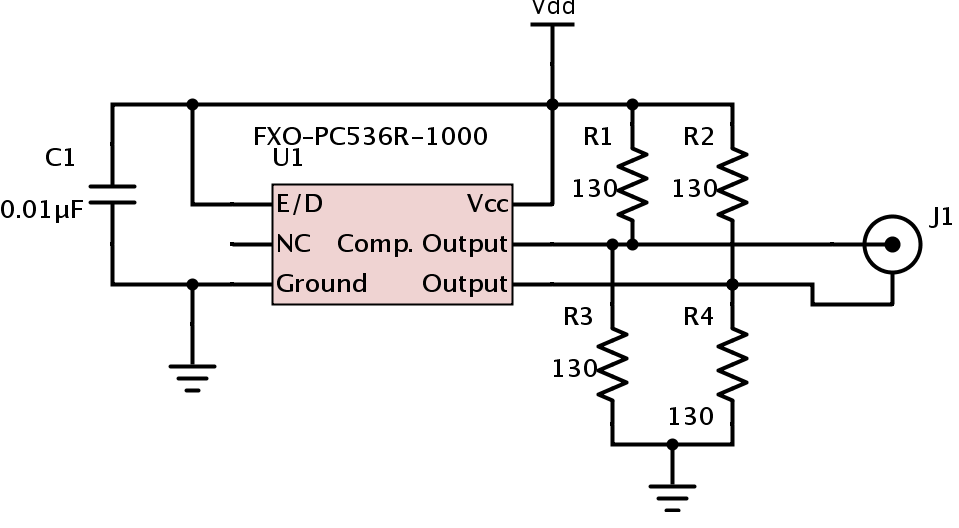
\includegraphics[width=0.75\textwidth]{Images/Schematics/1ghzclock_2.png}
\caption{Schematic of the 1 GHz clock. J1 is the 1 GHz output.}
\end{figure}

A frequency synthesizer, built by Stanley Hong \cite{hong}, uses this 1 GHz clock to synthesize a 80.25 MHz signal and an 80 MHz signal. The difference between these, a 250 Khz signal, is also generated, as it is necessary for signal processing.

Two RF amplifiers, purchased from Mini-Circuits (model ZHL-3A) amplify the RF signals +29.5 dBm to +32 dBm (approximately 1.5 Watts), the maximum drive power of the AOMs.

\subsection{Reference path}

%% TODO: Image of reference path setup

The reference path uses an adjustable focus fiber optic coupled collimator, and focuses it onto an AR-coated retroreflector. A retroreflector was used instead of a mirror to make alignment easier, as a retroreflector has no sensitivity to the angle offset between the collimated beam and its front surface. The collimator was initially used with an FC/APC fiber optic terminator, however, the $8^{\circ}$ face angle of FC/APC fiber connector reduced coupling efficiency dramatically. To fix this, a hybrid fiber patch cable was used, so that an FC/PC connector would connect to the collimator.

This setup was simulated with Zemax, as shown in Figure \ref{fig:reference_zemax}. Zemax predicted a single mode fiber coupling efficiency of -0.55 dB (as opposed to the -22.56 dB efficiency calculated with an FC/APC connector.)

\begin{figure}[h!]
\centering
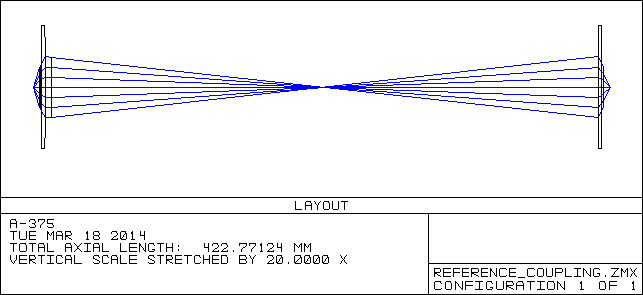
\includegraphics[width=0.75\textwidth]{Images/Zemax/RP-raytrace.png}
\caption{Zemax raytrace simulation of reference path.}
\end{figure}

The retroreflector was mounted on a non-motorized, single axis micropositioning stage, allowing the reference path length to be adjusted so that it aligns with the focal point of the sample path.

One consequence of using a retroreflector instead of a mirror is that the polarization of the beam is changed. This could be cause for concern if a future iteration of this system was ued for polarization sensitive imaging, however, the optical polarization is effectively randomized due to strain and compression in the optical fiber already.

\subsection{Sample path objective}

A graded index (or GRIN) lens was used. The GRIN lens is sold by Thorlabs, as a package that can be assembled to focus to a desired distance. This was fixed with Norland Optical Adhesive 68 and cured under UV light.

\begin{figure}[h!]
\centering
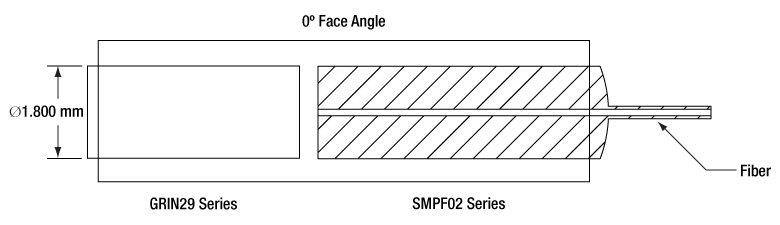
\includegraphics[width=1.0\textwidth]{Images/System/grin.png}
\caption{The GRIN lens assembly. \em{Image from Thorlabs.}}
\end{figure}

The size of the physical distance from the GRIN objective lens to the tissue under examination, referred to as the working distance $W$, is a tradeoff between the conveniences that having a large $W$ provides, the  transverse resolution, and the amplitude of scattered light.

%% scattered light amplitude

The solid angle $\Omega$ subtended by the GRIN lens is equal to

\begin{equation}
\Omega = 2 \pi (1 - \cos{\theta})
\end{equation}

where $\theta = \arctan{\frac{r_{grin}}{W}}$.

\begin{equation}
\Omega = 2 \pi \left(1 - \sqrt{\frac{W^2}{W^2 + r_{grin}^2}} \right)
\end{equation}

Assuming an isotropic scatterer, the fraction of optical power that will be recollected by the GRIN lens is equal to $ \left( \frac{\Omega}{4 \pi} \right)^2 $. As the GRIN lens used in this thesis has a radius of 0.9mm, this fraction may be written numerically as follows.

\begin{equation}
\frac{1}{4} \left( 1 - \sqrt{\frac{W^2}{W^2 + 0.81}} \right) ^ 2
\end{equation}

A plot of this value for working distances between 0 and 5 mm is shown in Figure \ref{fig:wd}.

\begin{figure}[h!]
\centering
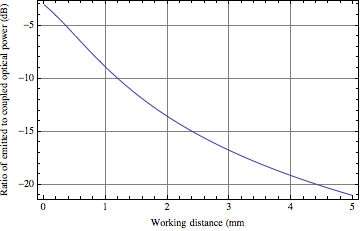
\includegraphics[width=0.6\textwidth]{Images/System/grin_scattering.png}
\caption{Captured light ratio as a function of working distance, in mm. \label{fig:wd}}
\end{figure}

As previously discussed in Equation \ref{eq:tres}, the axial resolution is given by:

\begin{equation} \label{eq:tres2}
\delta_x = 0.61 \frac{\lambda}{NA} \approx 1.22 \frac{\lambda W}{1.8 \mathrm{mm}} \approx W \cdot 0.888 \cdot 10^{-3} \;\;
\end{equation}

A working distance of 2 mm was choosen, resulting in a transverse resolution of 1.78 microns, and a reflection loss of -27.1 dB (again, assuming an isotropic scaterrer).

\section{Sample alignment apparatus}

%% solidworks images and mechanical design discussion

\begin{figure}[h!]
\centering
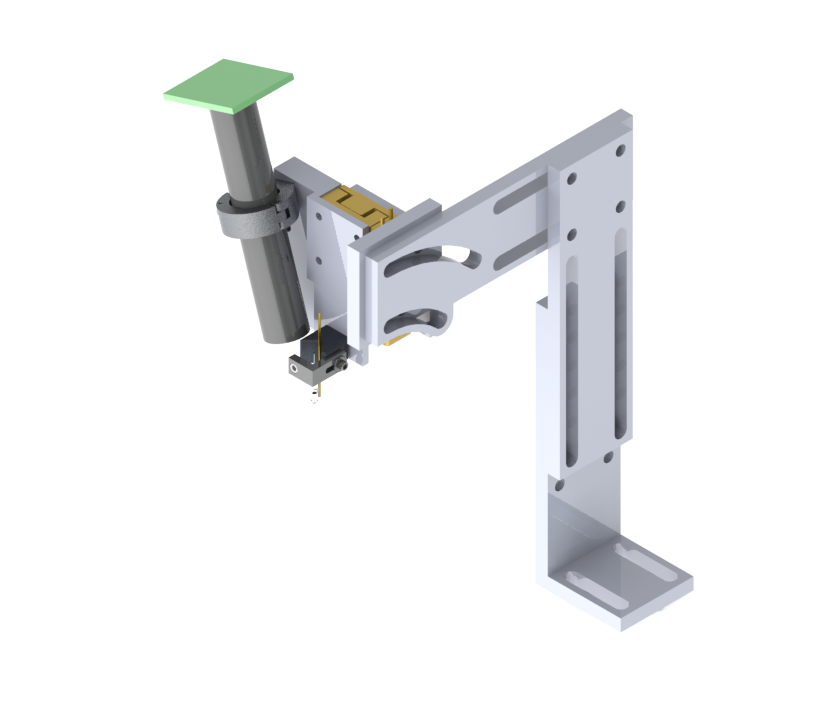
\includegraphics[width=1.0\textwidth]{Images/Alignment/new_d_2.png}
\caption{A SolidWorks model of the mechanical alignment apparatus.}
\end{figure}

The sample alignment apparatus is a mechanical device designed to satisfy several goals:

\begin{itemize}
	\item Securely hold the GRIN objective lens
	\item Move the GRIN objective along the direction of the optical axis with a precise motorized stage
	\item Allow the GRIN objective lens to be rotated a certain angle around its focal point
	\item Allow coarse adjustments for height and cantilever distance
	\item Provide a visible alignment aid beam
	\item Hold a small digital microscope for visual inspection of alignment
\end{itemize}

\subsection{Mechanical device for adjusting angle}

To control the angle, the z-stage is mounted on a horizontal aluminum cantilever, with two circularly concentric slots cut out. By screwing the stage mounting block into the slots, the angle can be adjusted around a fixed point. When the system is configured such that it is focused on this point, the operator is able to change the angle of axial movement without changing the current focal point, a helpful feature for alignment.

\begin{figure}[h!]
\centering
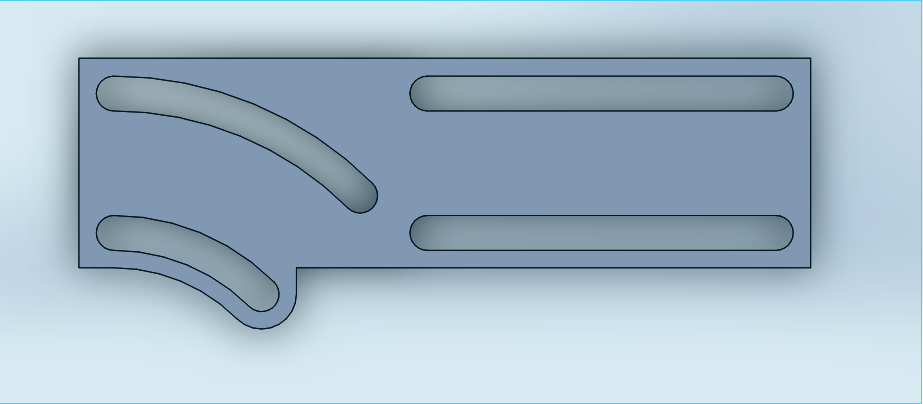
\includegraphics[width=1.0\textwidth]{Images/Alignment/horizontal_part.png}
\caption{The horizontal cantilever piece, with two slots allowing for angular adjustment.}
\end{figure}

The cantilever part was designed in SolidWorks and then milled on a CNC machine in the Edgerton Center Student Shop.

An L-shaped part was designed to hold the horizontal cantilever. Later, a vertical part was added to enable continuous adjustment of cantilever height, and to allow for a higher maximum height, necessary as a result of the clearance requirements of the Prior axial stage. These parts were milled by hand at the Edgerton Center Student Shop.

\subsection{Piezo motor stage for axial movement}

\begin{figure}[h!]
\centering
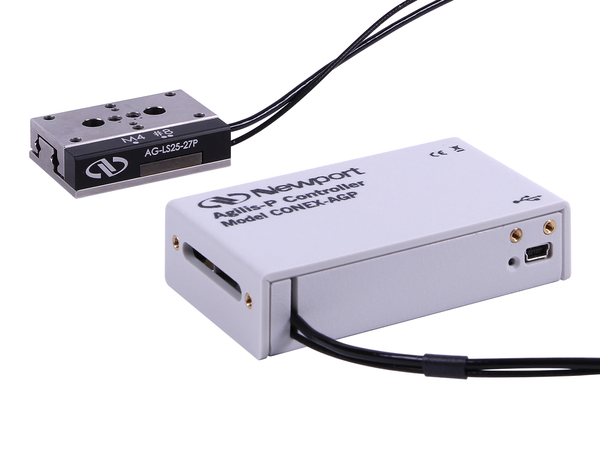
\includegraphics[width=0.48\textwidth]{Images/System/z-stage.jpg}
\caption{The piezo motor stage with controller.}
\end{figure}

\begin{table}[h!]
\centering
\begin{tabular}{ >{\bf}r | l}
Part number & CONEX-AG-LS25-27P\\
Travel range & 27mm  \\
Repeatability & 200 nm \\
Speed & 0.4mm / sec \\
Minimum incremental motion & 200nm \\
Price & \$1725 \\
\end{tabular}
\caption{Specifications for the axial piezo motor stage.}
\end{table}

To control $z$-axis scanning, a piezo-electric motorized stage was used. This stage uses an ``inchworm'' like drive method to control motion, and uses motion encoders with closed loop feedback to provide repeatable movements of up to 200 nm.

Unfortunately, this stage also has some drawbacks for an OCT application. Though the closed loop feedback allows for the stage to move precisely to any location, it's speed is not consistent during the motion. As a result, it is necessary to re-interpolate the data collected based on the actual position of the stage as it scans. This is discussed further in the signal processing section, Section \ref{sec:sig_proc}.

To capture information about the realtime position of the stage two approaches were used. The first involved repeatedly querieing the CONEX stage driver over TTY serial. While this was straightforward to accomplish and within the bounds of normal operation of the stage, it did not provide high enough resolution (in time) of the stages' position.

The second approach involved adding analog output from the stage encoder that could be captured by the analog-to-digital converter simultaneously with the interferometry signal. This involved ``hacking'' % should I use this word?
the controller.

\begin{figure}[h!]
\centering
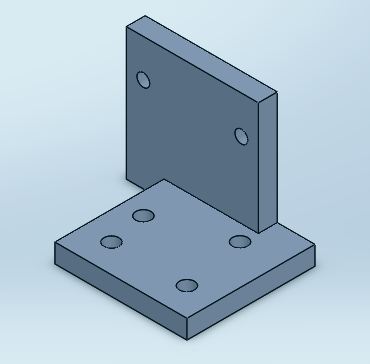
\includegraphics[width=0.48\textwidth]{Images/Alignment/angle_bracket2.png}
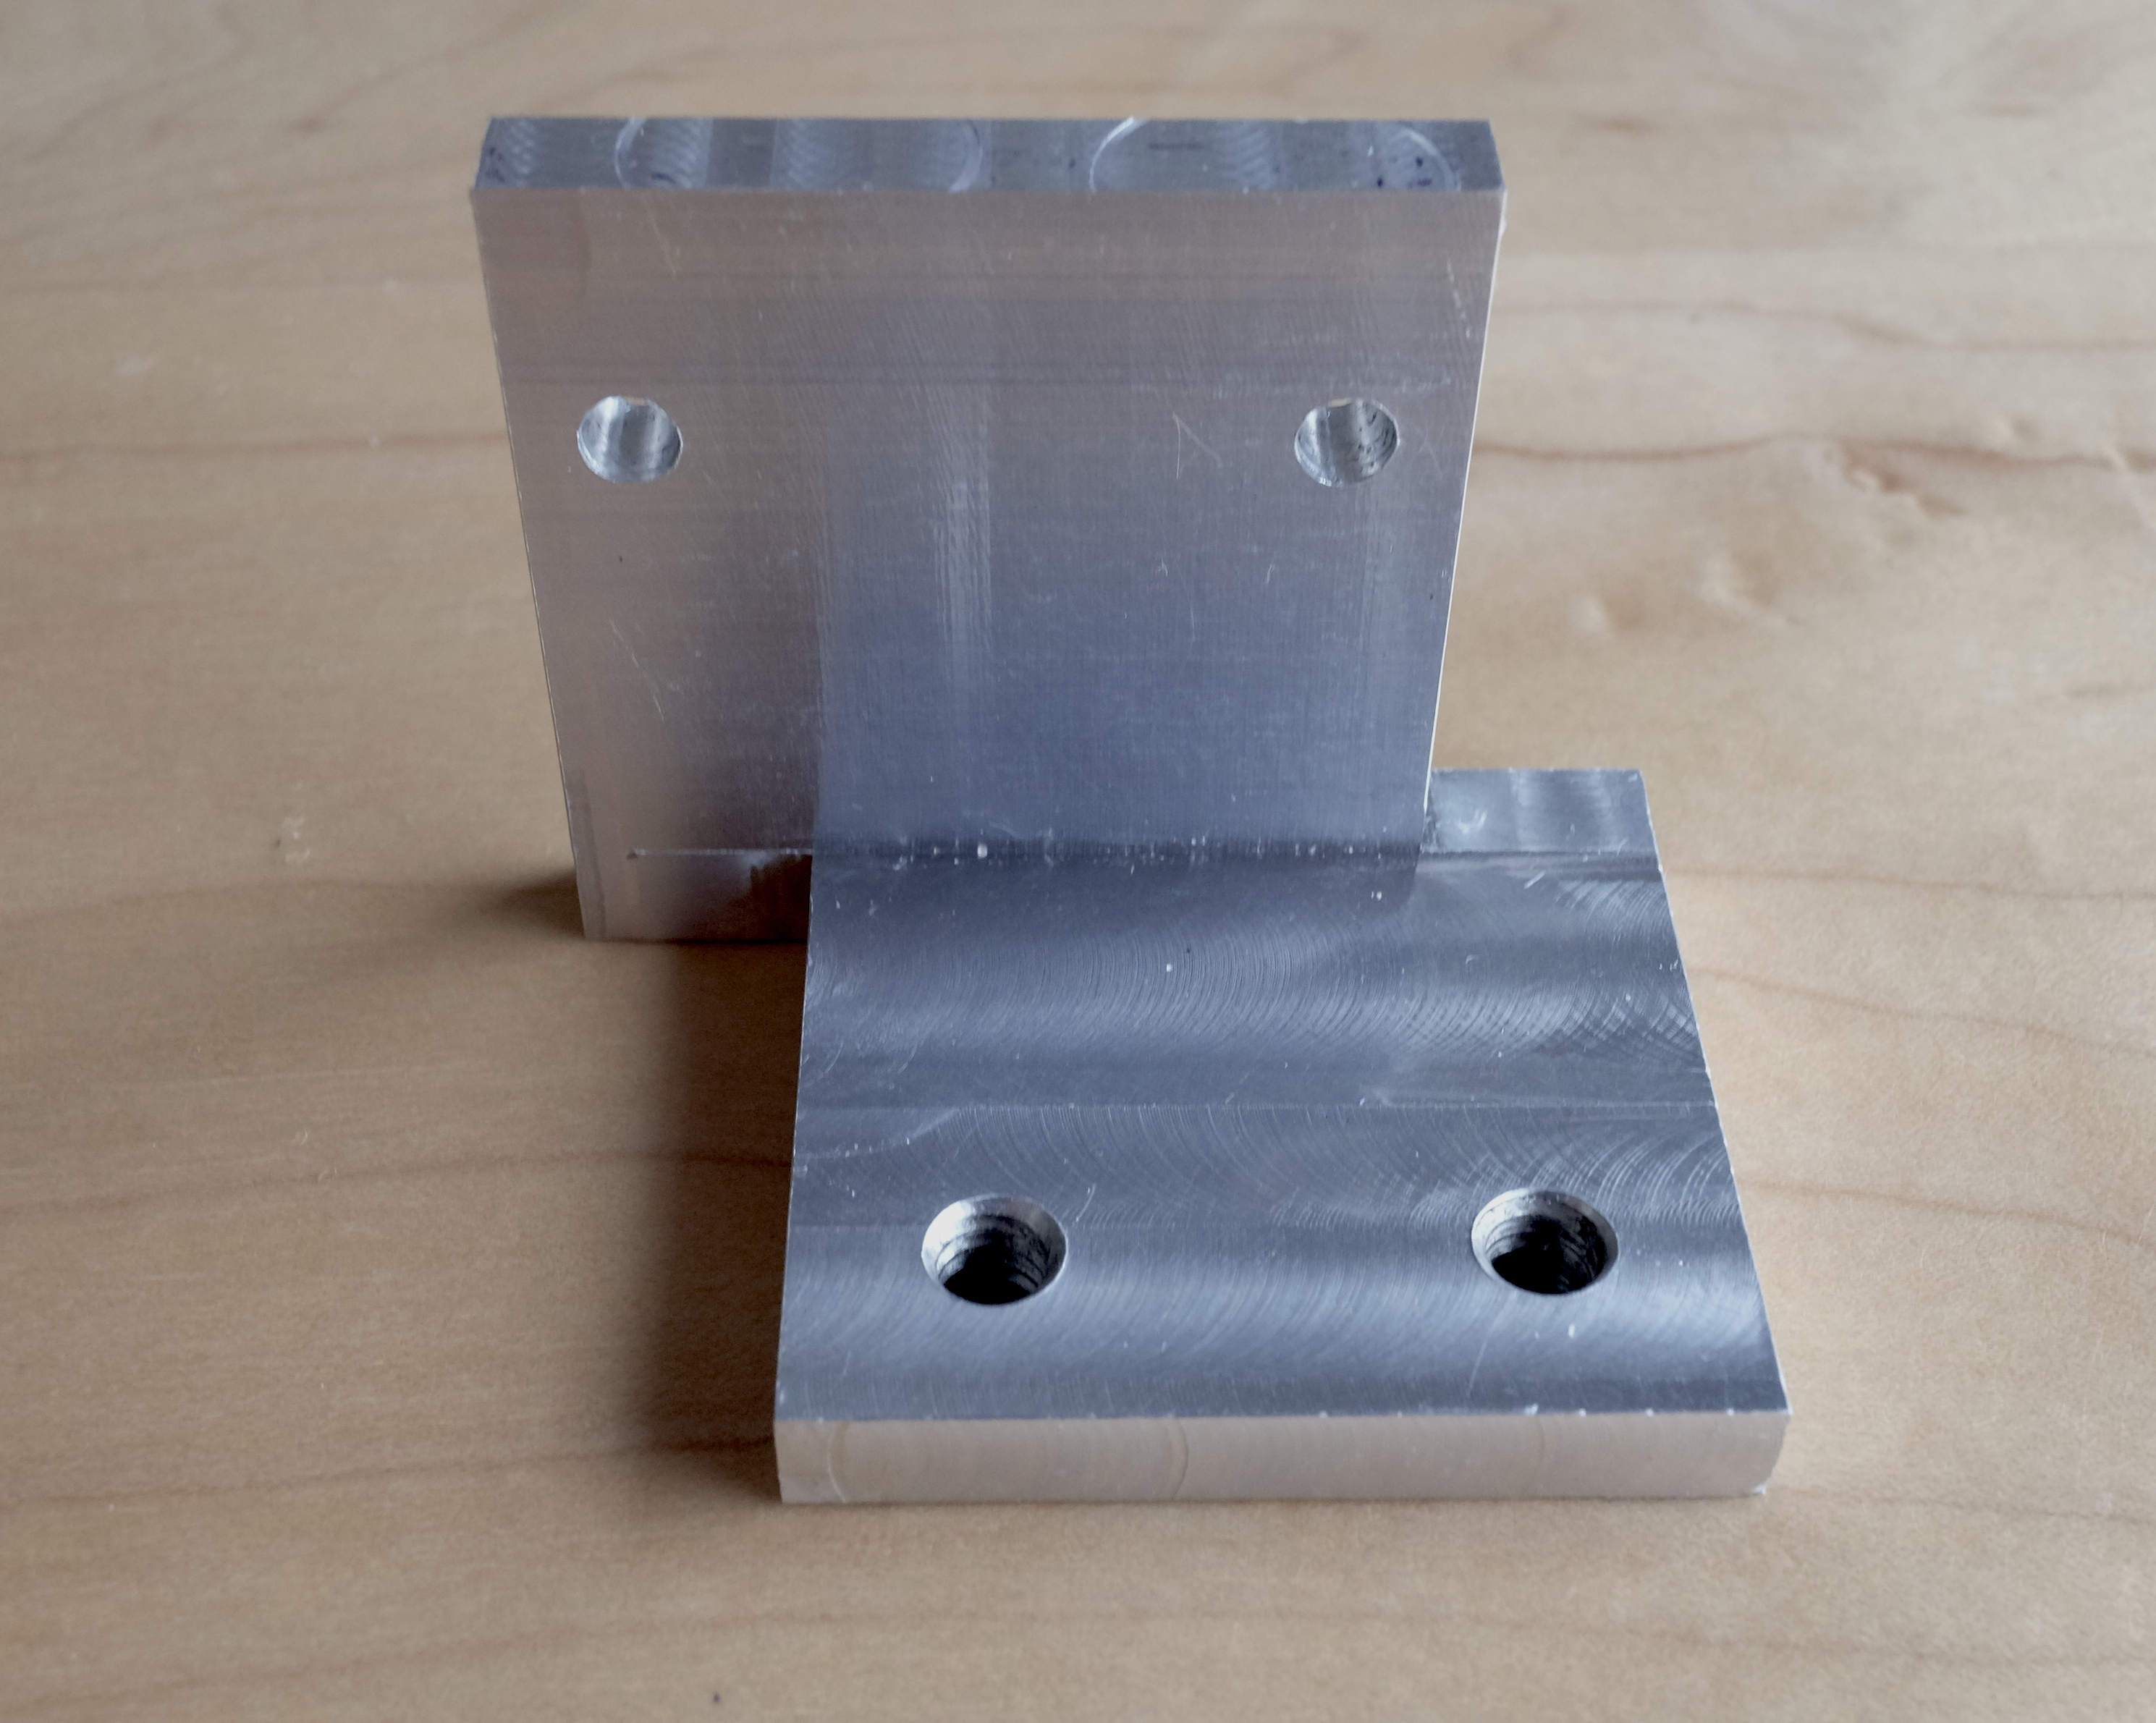
\includegraphics[width=0.48\textwidth]{Images/Alignment/angle_bracket.jpg}
\caption{This angled bracket mounts the piezo-motor stage to the horizontal cantilever shown above. The image on the right shows the bracket prior to the addition of stabilization bolts.}
\end{figure}

\subsection{Mounting the fiber and GRIN lens}

\begin{figure}[h!]
\centering
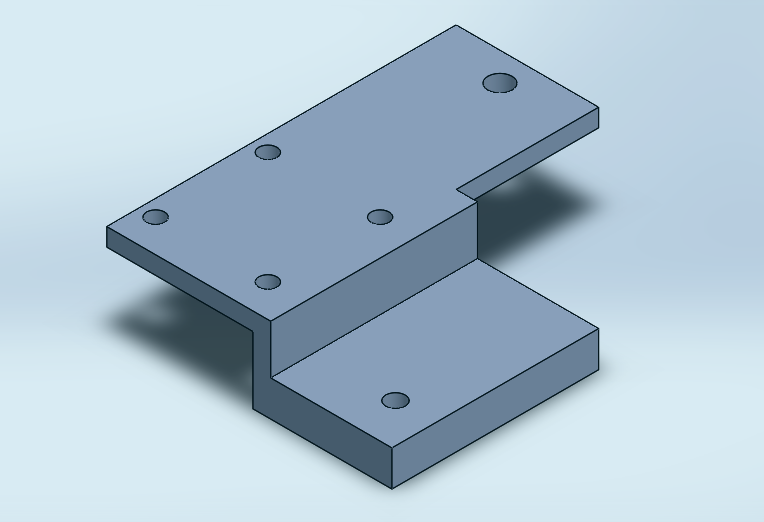
\includegraphics[width=0.75\textwidth]{Images/Alignment/mounting_plate.png}
\caption{This mounting bracket fastened to the z-stage and allowed the installation of a Thorlabs V-clamp.}
\end{figure}

To hold the fiber and its objective GRIN lens, a Thorlabs V-clamp was used. A custom part was designed in SolidWorks to connect to the piezo stage, allow the V-clamp to be mounted, and also to allow the digital microscope to be installed such that it could image the focal point of the GRIN lens. This part was designed in SolidWorks, and then milled by hand in the Edgerton Center Student Shop.

\subsection{Digital microscope for visual alignment}

%% Image of final microscope

In order to aid the alignment process, an optical microscope, with a digital CCD view finder, was constructed to observe the region imaged by the OCT process.

The design required a relatively large working distance (and correspondingly low numerical aperture), to allow the microscope to have an angle as close to the optical axis of the OCT objective lens as possible.

A CCD sensor from a Microsoft Xbox Live Vision web camera was used, due to its compact size, low cost, and use of the standard USB Video Class protocol (compatible with MATLAB and other image capture applications.) As the CCD has a quite small size, approximately 3x5mm (actual dimension specifications are not available), a low magnification was sufficient.

A MATLAB program was ued to optimize the working distance, while keeping the overall optical length within reasonable limits, and while working with a set of easily obtainable lenses, using a simple paraxial lens approximation. From this MATLAB program, a ZEMAX simulation model was constructed, using accurate models of the actual lenses from which the microscope would be constructed.

The microscope is composed of three lenses in two groups -- a 15mm spherical doublet (Edmund 45209) and a 20mm spherical singlet (Thorlabs LA1074). The lenses are mounted in $1/2$ inch $\diameter$ lens tubes. A 4mm diameter aperture, laser cut from opaque acrylic, was used to further reduce the pupil size, improving image quality at the cost of reducing light intensity.

\begin{figure}[h!]
\centering
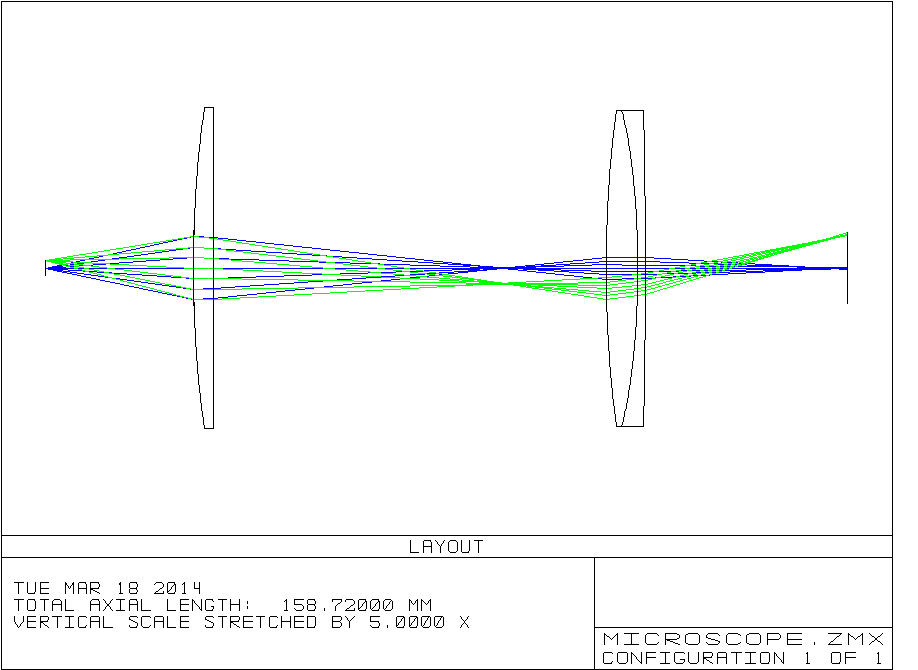
\includegraphics[width=0.8\textwidth]{Images/Microscope/microscope_layout_3.png}
\caption{A raytrace diagram of the microscope layout, simulated in ZEMAX.}
\end{figure}

\begin{figure}[h!]
\centering
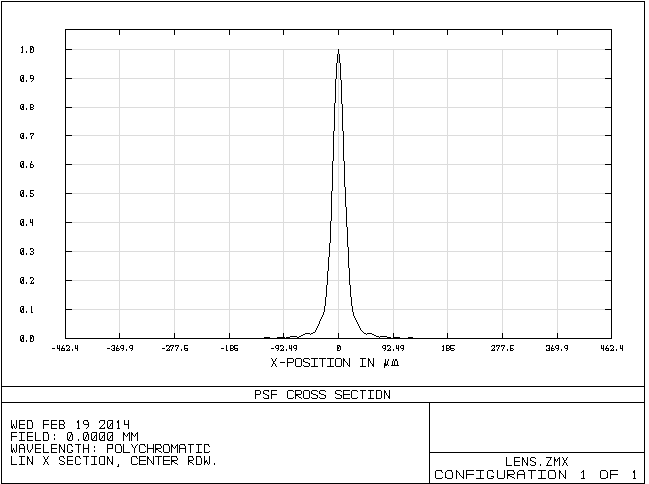
\includegraphics[width=0.8\textwidth]{Images/Microscope/microscope_psf.png}
\caption{The point spread function of the microscope, as simulated in ZEMAX. Note the actual performance was slightly better than in the simulation.}
\end{figure}

The performance was tested using a 1961 USAF Resolution Test Target, which showed that the microscope could resolve features down to 7.8 microns wide, and had a field of view of 1.16 mm $\times$ 0.87 mm, for a magnification of approximately 4$\times$.

\begin{figure}[h!]

\centering
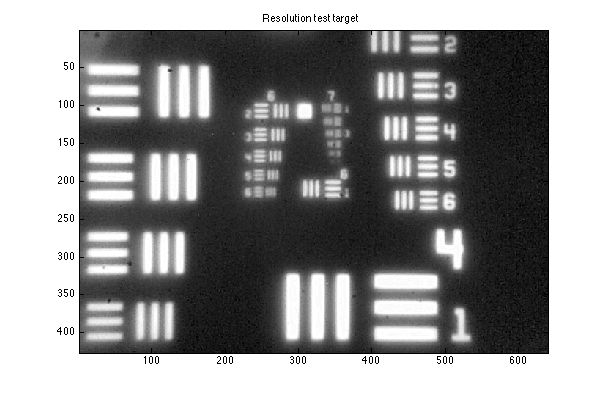
\includegraphics[width=1.0\textwidth]{Images/Microscope/target.png}
\caption{An image of a 1961 USAF Resolution Test Target, taken using the digital microscope. \label{fig:usaf}}
\end{figure}

While the performance of this microscope would not be considered ``great'' for any serious imaging applications (in particular, the contrast is quite poor, as evidenced by the ``haze'' around the bright regions in Figure \ref{fig:usaf}), it is sufficient for performing the basic alignment of the OCT appartus, and therefore is sufficient for the design requirements. Due to the nature of the microscope's application, the sample is not illuminated by transillumination, but instead by simply viewing the light scattered off of the sample from a bright LED source, mounted near the end of the microscope. Again, while this is not optimal for imaging applications, it meets the design requirements as an alignment microscope.

\subsection{Visible laser for assisting visual alignment}

%% Image of laser

The spectral responsivity of a silicon photo-sensor, like that used in the digital microscope CCD, falls sharply above 1000nm. As the optical source in this system is centered at 1310nm, it is difficult to view the spot produced by the focused infrared light. For this reason, a second optical source can be coupled into the GRIN lens.

For this purpose, an inexpensive 650nm laser diode is used. The output of the diode is collimated and coupled into an SMF-28e+ optical fiber, which can be attached through a FC-APC connector directly to the GRIN lens. This produces a highly visible laser spot that is helpful for aligning the start of an OCT scan.

%% Image of laser spot

\section{X-Y stage for sample movement}

To move in the transverse plane, the sample is placed on a stepper motor driven two axis stage. For this purpose, a Prior H101BX stage was used. While this stage is designed for use on a conventional upright microscope, some custom mounting hardware was designed and manufactured to allow it to stand freely. The stage is driven by a Prior H128 controller, which accepts commands over a serial port. Full specifications are in Table 2.4.

\begin{figure}[h!]
\centering
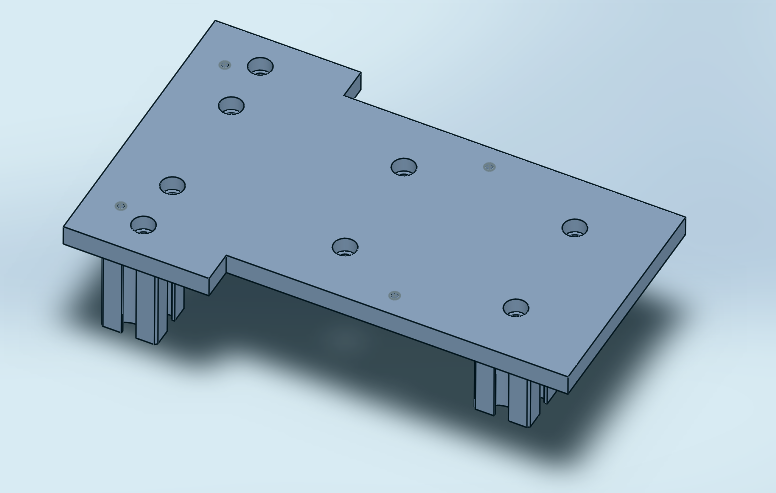
\includegraphics[width=0.75\textwidth]{Images/Alignment/x-y-mount.png}
\caption{The mounting plate designed to allow the Prior H101B microscope stage to stand freely. This was fabricated by laser cutting acrylic.}
\end{figure}

\begin{table}[h!]
\centering
\begin{tabular}{ >{\bf}r | l}
Part number & Prior H101BX \\
Travel range & 115 x 77 mm \\
Incremental step size & 40 nm \\
Bidirectional repeatability & 800 nm \\
Motor type & 200 Series Stepper \\
\end{tabular}
\caption{Specifications for the X-Y stage.}
\end{table} 


\section{Light detection and analog-to-digital conversion}

The light is detected by a Newport New Focus 2117-FC photodiode with an integrated trans-conductance amplifier. This photodiode has a sensitivity range of 800-1700nm, and a transimpedance gain of up to $18.8 \times 10^6 \;\; \mathrm{V}/\mathrm{A}$, with responsivity near $1 \mathrm{A}/\mathrm{W}$ at 1310 nm. Full specifications are detailed in Table \ref{table:pd}.

As the interference carrier signal is set at 500 KHz, the photodiode low-pass and high-pass filters are configured to pass signals between 300 Khz and 1 MHz.

\begin{figure}[h!]

\centering
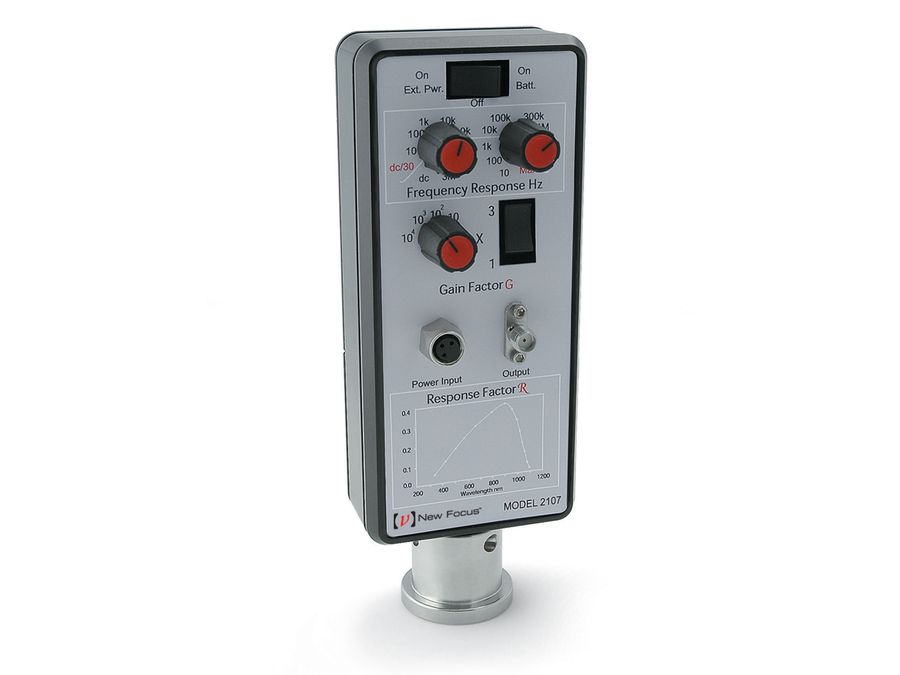
\includegraphics[width=0.6\textwidth]{Images/System/pd.jpg}
\caption{The Newport New Focus 2117-FC photodetector.}
\end{figure}

\begin{table}[h!]
\centering
\begin{tabular}{ >{\bf}r | l}
Part number & \\
Wavelength range & 800 - 1700 nm \\
Transimpedance gain & $18.8 \times 10^6 \mathrm{V/A}$ \\
Noise equivalent power & 0.4 $mathrm{pW}/\sqrt{\mathrm{Hz}}$ \\
Price & \$1390 \\
\end{tabular}
\caption{Specifications for the photo detector. \label{table:pd}}
\end{table}

The output from the photodiode is digitized by using an Interface Corporation PCI-3525 DAC/ADC card. Full specifications for this part are shown in Table \ref{table:dac}. Multiple PCI-3525 cards are daisy chained together to be able to capture $>2$ signals simultaneously. This is useful, as up to six signals may be of interest to capture: the photodiode output, the RF synthesizer difference frequency, the acoustic stimulus signal, and the two $z$-stage quadrature encoders.

To capture these signals, a program was written in C to communciate with the PCI-3525 cards. The source for this program may be found in Appendix \ref{app:pci3525}. As the photodiode filters frequencies above 1 MHz, a sampling frequency of 2.5 MHz was choosen to avoid frequency aliasing. The capture program allows the length of the signal captured to be specified as an input argument, allowing for application flexibility.

The PCI-3525 card can also be used to synthesize a low-frequency acoustic stimulus signal. This obviates the need to have a fifth input for the acoustic stimulus signal.

\begin{table}[h!]
\centering
\begin{tabular}{ >{\bf}r | l}
Part number & PCI-3525 \\
Bit depth & 12 \\
Sampling rate & 10 MS/s \\
\end{tabular}
\caption{Specifications for the DAC. \label{table:dac}}
\end{table}

\section{Signal processing}
\label{sec:sig_proc}

There are two distinct tasks that the OCT system will be required to and capable of performing. One is image generation -- creating a static 2D or 3D image of the sample. The other is motion analysis, capturing information about the movement of one specific area of a sample. The primary difference in these two tasks is that motion analysis requires a period of data to be sampled from one point, while image generation uses a continually scanning axis.

%% Mostly MATLAB and source code here. Theory behind the processing is introduced in Chapter 1

\subsection{Image generation}

An overview of the signal processing steps necessary on acquired data for a single z-axis sweep is shown in Figure \ref{fig:imagegen}.

\begin{figure}[h!]
\centering
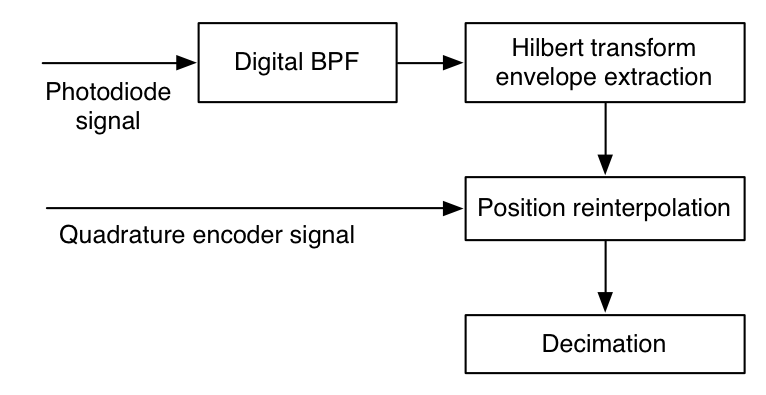
\includegraphics[width=0.65\textwidth]{Images/Background/image_analysis.png}
\caption{A block diagram overview of the steps necessary for image generation. \label{fig:imagegen}}
\end{figure}

First, the captured signal is bandpassed with a smaller passband than is practical with analog filters. Next, the Hilbert transform is used to extract the envelope of the signal. Using data from the quadrature encoders of the $z$-axis stage, this envelope is reinterpolated to be a function of space instead of time. As the envelope is much more slowly varying than the original 500 KHz signal, it can be decimated to the size desired for the final image. This process is repeated for each captured line to assemble the full 2D or 3D image.

This is implemented in MATLAB, code for which may be found in the Appendicies.

\subsection{Motion analysis}

An overview of the signal processing steps necessary to perform on acquired data to estimate motion parameters is shown in Figure \ref{fig:motion_analysis_block_diagram}.

\begin{figure}[h!]
\centering
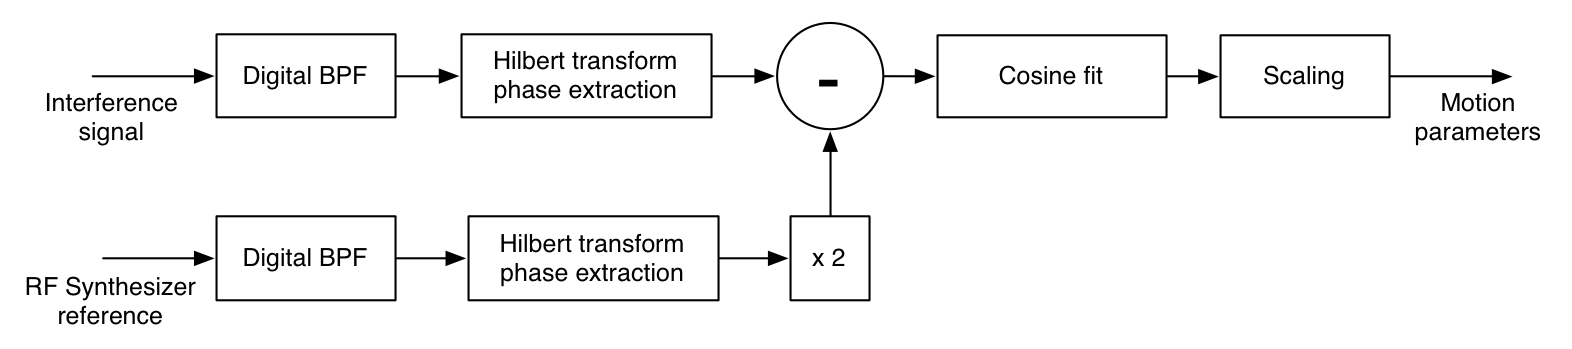
\includegraphics[width=1.0\textwidth]{Images/Background/motion_process.png}
\caption{The motion analysis signal flow. \label{fig:motion_analysis_block_diagram}}
\end{figure}

This process is the same as derived mathematically in Section \ref{sec:sigproc_mo_anal}. First, the Hilbert transform is used to estimate the instantaneous phase of the photodiode interference signal, and of the 250 KHz reference output from the RF synthesizer. The difference between the 500 KHz phase signal, and twice the 250 KHz phase signal is periodically varying when the frequency of the 500 KHz signal varies periodically (as is the case when light is scattered from a moving sample.) A least squares fitter is ued to fit a sinusoid to this periodically varying phase, from which the amplitude of the motion and the phase of the motion may be estimated. This provides an estimate of the motion parameters at a single point in the sample. This process can be repeated for as many points are desired, or for an entire array of points in order to generate an image of motion amplitude and phase in a tissue.

This analysis is implemented in MATLAB, code for which may be found in the Appendices.

%%%%%%%%%%%%%%%%%%%%%%%%%%%%%%%%%%%%
%%%%%% SECTION 2 PERFORMANCE %%%%%%%
%%%%%%%%%%%%%%%%%%%%%%%%%%%%%%%%%%%%
\section{Theoretical performance predictions}
\label{sec:theory_res}

\subsection{Axial resolution}
\label{sec:axial_res}

Axial resolution is limited by the coherence length of the optical source, as derived in Equation \ref{eq:ares} in Chapter 1. This result is repeated below:

\begin{equation} \label{eq:ares2}
\delta_z = l_c = \frac{2 \ln{2}}{\pi} \frac{\lambda_0^2}{\Delta \lambda}
\end{equation}

The specifications for the optical source used in this project were not precisely equivalent to the measured performance of the actual source. The actual -3dB bandiwdth was 86.3 nm, whereas the specified was 100 nm. Additionally, the actual power output was 7.00 mW, whereas the specified was 10 mW. The results of optical spectrum measurement for this source is shown below.

% Optical spectrum analyzer graph
\begin{figure}[h!]
\centering
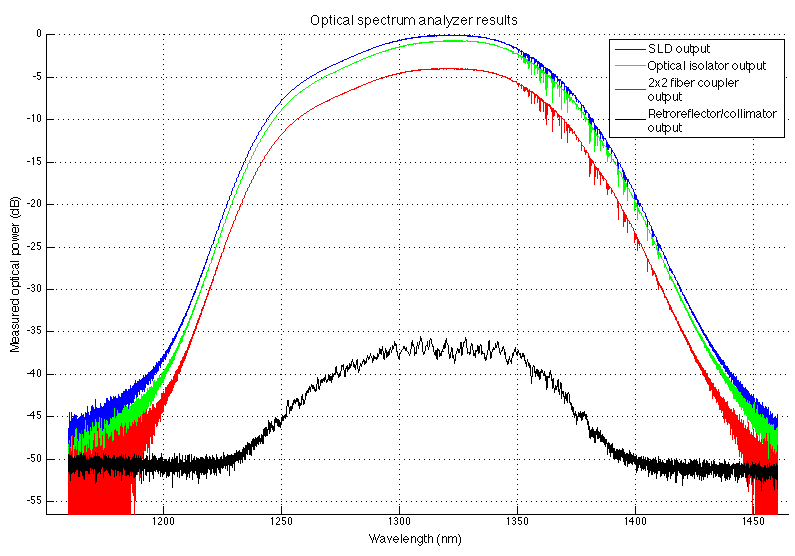
\includegraphics[width=1.0\textwidth]{Images/System/osa.png}
\caption{Optical spectrum analyzer results for the outputs of four critical parts in the OCT system. Due to a different experimental setup, the power levels measured in retro-reflector collimation are not representative of the actual system, and are clearly heavily affected by the noise floor of the optical spectrum analyzer. \label{fig:osa}}
\end{figure}

The slightly smaller bandwidth results in a slightly inferior axial resolution prediction of 8.77 microns. The designed axial resolution (based on data from the Exalos datasheet) was 7.57 microns.

This resolution is not adversally impacted by any other optical components in the system. The results of optical spectrum measurement at the output of several key components in the OCT system are shown in Figure \ref{fig:osa}.

% More OSA graphs?

\subsection{Transverse resolution}
\label{sec:transverse_res}

The maximum achievable resolution in the transverse direction is determined by the diffraction limit, as discussed in Chapter 1.

\begin{equation} \label{eq:tres2}
d = n\frac{\lambda D}{2f}
\end{equation}

where $D$ is the diameter of the entrance aperture, and $f$ is the working distance of the lens (distance to focal point). For the system described above, this evaluates to a diffraction limit of 590 nanometers.

Using ZEMAX Optical Design Software, and files provided from Thorlabs, the manufacturer of the GRIN lens, a more accurate simulation was created of the objective lens performance. Here, it was found to be diffraction limited when an object was on the optical axis (as is the case when emerging from an optical fiber).

\begin{figure}[h!]
\centering
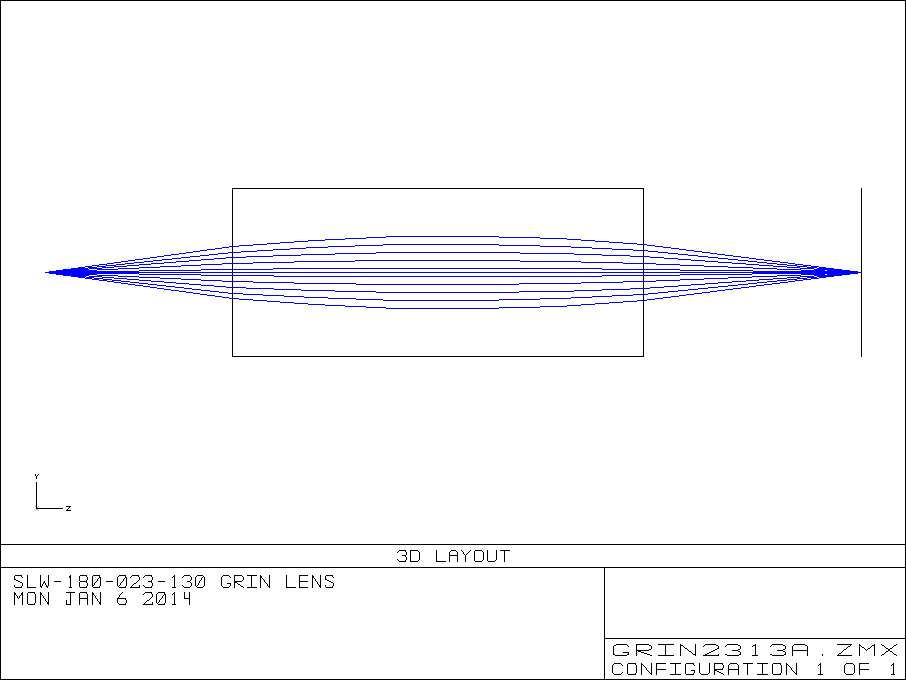
\includegraphics[width=0.75\textwidth]{Images/Zemax/GRO-raytrace.png}
\caption{A ZEMAX raytrace showing the path of light through the GRIN lens. Light emerges from the SMF-28e fiber (NA = 0.14) on the left, and is focused to a point on the right.}
\end{figure}

\begin{figure}[h!]
\centering
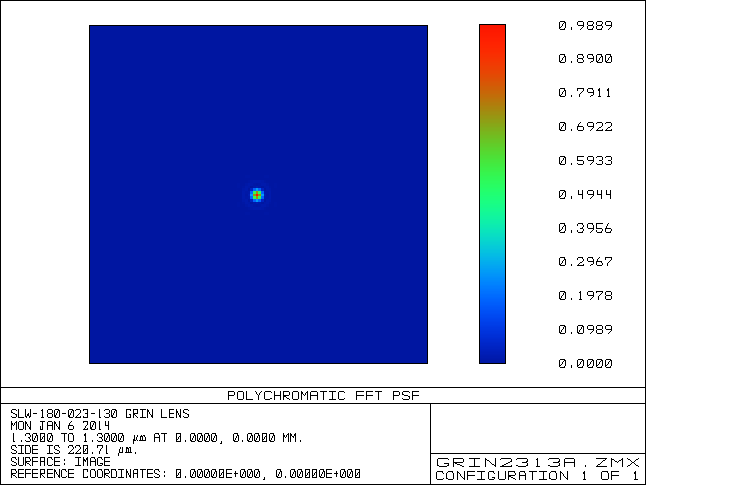
\includegraphics[width=0.75\textwidth]{Images/Zemax/GRO-psf.png}
\caption{The 2D PSF of the GRIN lens objective system. The area shown is 220 microns on each side.}
\end{figure}

\begin{figure}[h!]
\centering
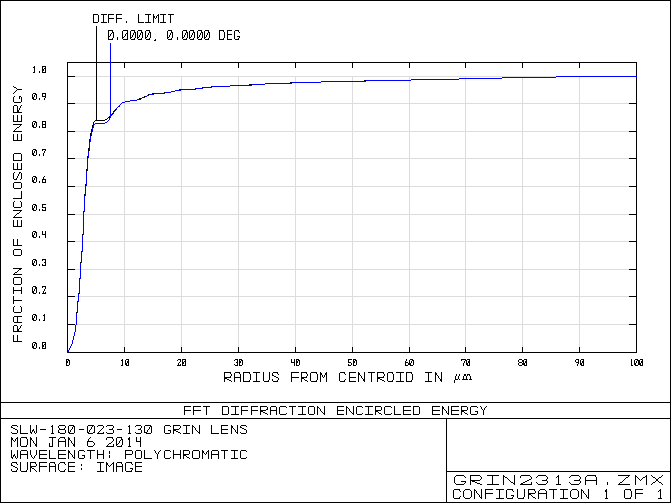
\includegraphics[width=0.75\textwidth]{Images/Zemax/GRO-encircledenergy.png}
\caption{A graph of the energy encircled at a given radius for the actual lens, and for diffraction only. This shows performance that is very nearly diffraction limited.}
\end{figure}

\subsection{Motion resolution}
\label{sec:motion_res}

The motion resolution is dependent on the spectral noise floor of the captured signal.
\chapter{System characterization}

\section{Verification of axial resolution}

\subsection{Results without AOMs}

\subsection{Results with AOMs}

\section{Verification of transverse resolution}

\section{Verification of motion resolution}

\section{Resolution of motion differentiation}
%\chapter{Results and conclusion}

In this chapter, results obtained with the FO-DOCM device on actual cochlear tissues will be shown. The shortcomings and successes of the apparatus will be detailed, and conclusions will be drawn.


%\appendix
%\chapter{Tables}

\begin{table}
\caption{Armadillos}
\label{arm:table}
\begin{center}
\begin{tabular}{||l|l||}\hline
Armadillos & are \\\hline
our	   & friends \\\hline
\end{tabular}
\end{center}
\end{table}

\clearpage
\newpage

%\chapter{Figures}

\vspace*{-3in}

\begin{figure}
\vspace{2.4in}
\caption{Armadillo slaying lawyer.}
\label{arm:fig1}
\end{figure}
\clearpage
\newpage

\begin{figure}
\vspace{2.4in}
\caption{Armadillo eradicating national debt.}
\label{arm:fig2}
\end{figure}
\clearpage
\newpage

%% This defines the bibliography file (main.bib) and the bibliography style.
%% If you want to create a bibliography file by hand, change the contents of
%% this file to a `thebibliography' environment.  For more information 
%% see section 4.3 of the LaTeX manual.
\begin{singlespace}
\bibliography{main}
\bibliographystyle{plain}
\end{singlespace}

\end{document}

